\chapter{Scintillatori}
Gli scintillatori si basano sull'emissione luminosa da parte di atomi eccitati:
una particella ionizzante deposita la propria energia sul materiale causando una eccitazione atomica o molecolare e, in seguito,
emissione di radiazione luminosa.
Gli scintillatori hanno usi multipli:
\begin{itemize}
\item Spettroscopia $\gamma$
\item Calorimetria
\item Sistema T.O.F.
\item Sistema di trigger
\item Sistema di veto
\item Traccianti
\end{itemize} 
Possono essere divisi in due macrocategorie:
\begin{itemize}
\item Inorganici, caratterizzati da una buona resa in luce (e quindi una maggiore efficienza), ma anche pi\`u lenti
\item Organici, con una resa in luce minore, ma una maggiore velocit\`a
\end{itemize}
\section{Meccanismo di scintillazione}
\subsection{Scintillatori inorganici}
\begin{figure}[htb]
\begin{center}
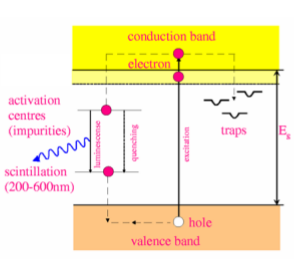
\includegraphics{./Immagini/LivelliEnergeticiScintillatore.png}
\caption{Livelli energetici in uno scintillatore inorganico}
\label{fig:livInorganico}
\end{center}
\end{figure}
La figura~\ref{fig:livInorganico} mostra il funzionamento di uno scintillatore inorganico.\\
In uno scintillatore organico per stimolare le attivazioni vengono introdotte delle impurezze, quando un elettrone viene portato
dalla banda di valenza a quella di conduzione entro qualche ns si ricombina con la lacuna emettendo radiazione.
Per via delle impurezze a volte accade che l'elettrone si vada a posizionare in un livello energetico dell'impurezza, questo
livello energetico ''trappola`` pu\`o richiedere tempi lunghi fino alle centinaia di ms per la diseccitazione. 
In questo caso avviene una fosforescenza.\\
Questi tipi di scintillatori hanno un elevato $Z$ e alta densit\`a, rendendoli adatti alla rivelazione di particelle cariche e raggi $\gamma$.
\subsection{Scintillatori organici}
\begin{figure}[htb]
\begin{center}
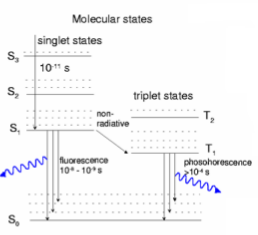
\includegraphics[scale=1.00]{./Immagini/LivelliEnergeticiScintillatoreOrganico.png}
\caption{Livelli energetici di uno scintillatore organico}
\label{fig:livOrganico}
\end{center}
\end{figure}
Gli scintillatori organici si basano sull'eccitazione di molecole di tipo organico, in particolare queste molecole sono caratterizzate
da orbitali molecolari di tipo $\pi$ tra le molecole di carbonio che possono essere stimolati per emettere luce nell'ultravioletto.\\
Posso avere scintillatori a monocristalli, liquidi o plastici a seconda dell'uso che si intende fare.\\
Il grande pregio di questo tipo di rivelatore sta nella velocit\`a di risposta che \`e nei ns.
Sono, inoltre, molto economici.
\section{Caratteristiche di uno scintillatore ideale}
\begin{enumerate}
\item Alta efficienza di scintillazione
\item Conversione lineare $S = E \cdot L$
\item Trasparenza 
\item Tempo di emissione breve
\item Buone propriet\`a ottiche e meccaniche. Buona maneggiabilit\`a.
\item Indice di rifrazione simile al vetro, per evitare riflessione totale.
\end{enumerate}
\subsection{Efficienza di scintillazione}
Uno scintillazione ideale dovrebbe avere un elevato $S$:
\begin{equation*}
S = \frac{L}{E} 
\end{equation*}
con $L$ energia luminosa e $E$ energia entrante.
Normalmente questo fattore \`e molto contenuto, nell'ordine del 10\%, per il NaI vale 12\% (il migliore).
Il resto dell'energia finisce in fononi e ionizzazione.\\
La \textbf{formula di Birks} (vale sono per gli scintillatori organici) afferma:
\begin{equation*}
\frac{dL}{dx} = \frac{S \frac{dE}{dx}}{1 + k_B \, \frac{dE}{dx}}
\end{equation*}
con $k_B$ costante di proporzionalit\`a di Birks.
Per le particelle $\alpha$ $\frac{dE}{dx}$ \`e molto grande per cui si ricava $\frac{dL}{dx} = \frac{S}{k_B}$, per gli elettroni
$\frac{dE}{dx}$ \`e piccolo per cui il termine al denominatore pu\`o essere approssimato a 1, ottenendo $L = S \cdot E$.\\
L'efficienza dipende dalla temperatura (fig~\ref{fig:traspInorganici}), dalle impurezze (per via del quenching) e si deteriora con il tempo.
\begin{figure}[htbp]
\begin{center}
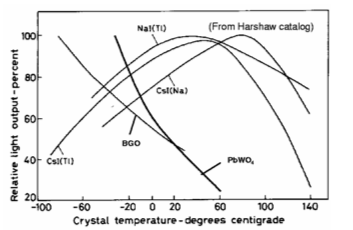
\includegraphics[scale=1]{./Immagini/TrasparenzaOrganici.png}
\caption{Andamento della trasparenza con la temperatura, esistono temperature ottimali.}
\label{fig:traspInorganici}
\end{center}
\end{figure}
\subsection{Linearit\`a}
La relazione $S = E \cdot L$ deve essere lineare, in particolare $S$ non dovrebbe dipendere dalla posizione dello scintillatore.
In generale $S$ dipende dalla particella, come si \`e visto dalla formula di Birks e per particelle che disperdono molta energia la relazione perde in linearit\`a:
per elettroni sufficientemente energetici (sopra il centinaio di keV) la relazione \`e lineare, per protoni o $\alpha$ non \`e lineare ad alte energie (si osservano
effetti di quenching tra molecole).
\subsection{Trasparenza}
\`E importante che lo spettro di assorbimento si sovrapponga il meno possibile con lo spettro di emissione, in modo da avere un materiale trasparente ai fotoni e
permettere ad essi di uscire dal materiale scintillante.
\subsection{Tempo di emissione}
Per avere un'elevata risoluzione temporale \`e necessario che la costante di tempo $\tau$ sia molto breve:
\begin{equation*}
I(t) = I_0 e^{-\frac{t}{\tau_0}} + I_1 e^{-\frac{t}{\tau_1}} - I_0 e^{-\frac{t}{\tau_p}}
\end{equation*}
con $\tau_0$ tempo di scintillazione, $\tau_1$ tempo di fosforescenza e fluorescenza ritardata e $\tau_p$ tempo per il popolamento dei livelli eccitati.
\subsection{Proprieta ottiche e meccaniche}
Per propriet\`a ottiche si intende che la geometria dello scintillatore deve essere tale da avere una buona raccolta di luce, per questo \`e necessario
che i cristalli abbiano buone propriet\`a meccaniche: essi devono essere, infatti, di dimensioni e forma variabili secondo le necessit\`a.\\
Per quanto riguarda la maneggevolezza alcuni cristalli sono igroscopici, ovvero assorbono l'umidit\`a dell'aria, per questo devono essere isolati e sotto vuoto, e possono
essere fragili.
\section{La raccolta della luce}
Quando uno scintillatore emette luce, essa viene diffusa in modo isotropico, per questo motivo \`e importante avere un buon meccanismo di raccolta della luce.
Per evitare che la luce esca dal cristallo senza andare sul fotocatodo si usa il meccanismo della riflessione totale:
\begin{equation*}
\text{sin} \, \theta_c = \frac{n_1}{n_0}
\end{equation*}
Questo permette di avere minori perdite alla superficie (l'efficienza \`e sul 80\%) tuttavia rende difficoltosa la trasmissione del segnale al fotocatodo.
Per questo sulla superficie rivolta verso il fotocatodo viene posto un materiale di accoppiamento, ovvero un materiale a indice di rifrazione intermedio, come
del grasso ottico o del silicone.
Siccome il fotocatodo lavora con campi elettrici e magnetici intensi \`e necessario porlo ad una certa distanza dal cristallo, pe questo
\`e necessario guidare la luce verso il fotocatodo mediante l'uso di \textbf{guide di luce}, fibre a geometria cilindrica che trasportano la radiazione luminosa.
\section{Il fotocatodo}
Il fotocatodo ha il ruolo di emettere fotoelettroni quando fotoni di sufficiente energia incidono su di esso.
Questo dispositivo non \`e sensibile a tutta la radiazione luminosa: 
per ottenere l'emissione di un fotoelettrone \`e necessario che il fotone incidente
abbia energia sufficiente a portare un elettrone dalla banda di valenza del materiale alla
banda di conduzione ed a farlo uscire dalla superficie del fotocatodo (generalmente $E_{\gamma} > 2$ eV).
Per questo motivo il fotocatodo \`e in grado di rivelare solo una certa porzione dello spettro
luminoso, in genere a partire dal giallo-verde, in base al materiale che lo compone. \\
Per costruire i fotocatodi si utilizzano dei semiconduttori drogati ad affinit\`a elettronica negativa, ad esempio GaP drogato di tipo p con zinco.\\
Quando un elettrone viene portato in banda di conduzione, esso inizia ad eccitare i fononi del cristallo,
disperdendo la propria energia e raggiungendo (generalmente entro 1 ps) il fondo della banda.
Una volta che si trova in questo stato, l'elettrone impiega un tempo nell'ordine dei 100 ps per ricombinarsi con una
lacuna, tornando in banda di valenza.
L'energia sul fondo della banda di conduzione non \`e sufficiente per permettere agli elettroni di fuggire dal fotocatodo:
tra il materiale ed il vuoto esiste, infatti, una barriera di potenziale (detta affinit\`a elettronica) che impedisce agli elettroni di lasciare il semiconduttore.
Gli unici elettroni ad avere energia sufficiente per superare la barriera sono quelli che
hanno eccitato pochi fononi, per cui gli elettroni possiedono un tempo di 1 ps per lasciare il fotocatodo.
Questo tempo \`e molto breve e pone seri limiti allo spessore del materiale, in quanto gli elettroni possono percorrere poco spazio.
Per aumentare l'efficienza dei fotocatodi, essi vengono contruiti in modo da avere un'affinit\`a elettronica negativa e permettere agli elettroni sul fondo della banda di conduzione di avere energia sufficiente per fuggire.
Questo effetto viene ottenuto deponendo uno strato monoatomico di un materiale elettropositivo (ad esempio il cesio) sulla superficie del dispositivo:
poich\'e gli elettroni del cesio sono poco legati, essi vengono attratti dalle lacune del semiconduttore, ionizzando lo strato ed abbassando l'affinit\`a elettronica.
\subsection{Fabbricazione dei fotocatodi}
Esistono 2 categorie di fotocatodi, quelli opachi, con uno spessore maggiore della profondit\`a di fuga degli elettroni e quelli semitrasparenti.
In quelli opachi gli elettroni vengono prelevati dallo stesso lato in cui la luce incide sul materiale, in quelli semitrasparenti avviene l'opposto, in quanto la luce
riesce a raggiungere l'altro estremo del materiale.\\
Ad ogni modo \`e fondamentale che i fotocatodi abbiano uno spessore uniforme, per avere un estrazione uniforme indipendentemente dalla regione colpita dalla radiazione.
Esistono fotocatodi bialcalini o multialcalini a seconda della risposta alla radiazione che si desidera ottenere.
\section{Il fotomoltiplicatore}
\begin{figure}[htbp]
\begin{center}
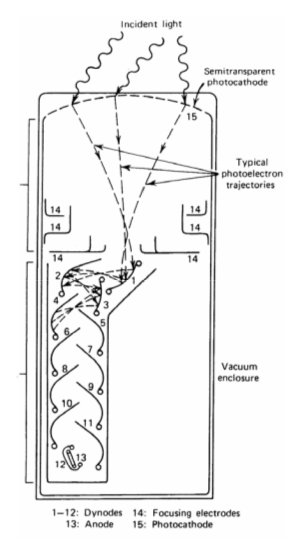
\includegraphics[scale=0.8]{./Immagini/Fotomoltiplicatore.png}
\caption{Schema di un fotomoltiplicatore}
\label{fig:fotomolt}
\end{center}
\end{figure}
Il rendimento quantico di un fotomoltiplicatore viene definito come:
\begin{equation*}
\text{Q.E.} = \frac{N_{pe}}{N_{fot}} \approx 20\% - 30\%
\end{equation*}
esso dipende dalla lunghezza d'onda del fotone incidente.
Un fotomoltiplicatore si basa sulla moltiplicazione di fotoelettroni attraverso stadi successivi chiamati \textbf{dinodi}.
Quando un fotoelettrone lascia il fotocatodo, esso viene accelerato da un potenziale verso i dinodi, l'urto con i dinodi libera della carica che
attraverso ulteriori urti viene moltiplicata e, infine, raccolta sull'anodo, producendo un segnale elettrico misurabile.
Tipicamente ogni urto con un dinodo porta ad un guadagno da 3 a 50 elettroni, il prodotto di tutti i guadagni da il guadagno globale.
Ad esempio 10 dinodi con guadagno $g=4$ moltiplicheranno di un fattore $G=4^{10}\approx 10^6$.\\
Di particolare importanza \`e il rumore termoionico dovuto ad emissioni termiche di elettroni da parte del fotocatodo:
a 300 K, $k_b T$ vale circa 25 meV, tuttavia per le code della distribuzione si ha che alcuni elettroni hanno un energia maggiore del lavoro di estrazione, 
causando falsi segnali.
Per questo motivo \`e necessario tenere il fotocatodo freddo, in genere per i semiconduttori si hanno dai 100 ai 10000 elettroni/cm$^2$ e s.\\
La \textbf{risoluzione energetica} \`e fortemente dominata dalla moltiplicazione al primo dinodo, dove gli elettroni sono pochi e 
$\frac{\sigma_E}{E} \propto \frac{1}{\sqrt{n}}$.
\subsection{I dinodi}
Supponiamo che un fotone liberi un elettrone e che esso sia accelerato da una differenza di potenziale di 100 V verso il primo dinodo.
Essendo il gap nell'ordine dei 2-3 eV, verranno eccitati circa 30 elettroni, di cui solo 4-5 usciranno dal dinodo per andare verso lo stadio successivo.
Aumentando il potenziale la quantit\`a di elettroni liberati cresce, tuttavia essi verranno liberati pi\`u in profondit\`a.
Per questo motivo esiste un valore ottimale per il potenziale di accelerazione.\\
In genere per i dinodi standard il valore di moltiplicazione \`e 5, per i materiali ad affinit\`a elettronica negativa si possono raggiungere fattori di moltiplicazione
pari a 20-30.
\section{Alimentazione del sistema a dinodi}
Chiaramente \`e necessario che la tensione dell'anodo sia maggiore di quella del fotocatodo, questo pu\`o essere ottenuto in due modi:
\begin{itemize}
\item fotocatodo a massa e anodo a tensione positiva
\item fotocatodo a tensione negativa e anodo a massa
\end{itemize}
Per alimentare i vari stadi di moltiplicazione \`e comodo usare un partitore resistivo (figura~\ref{fig:partitoreDinodi}).
\begin{figure}[htb]
\begin{center}
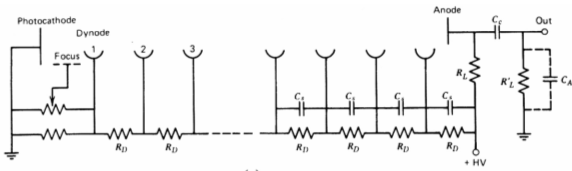
\includegraphics[scale=0.80]{./Immagini/PartitoreDinodi.png}
\caption{Esempio di partitore resistivo per i dinodi}
\label{fig:partitoreDinodi}
\end{center}
\end{figure}
Chiaramente un sistema di questo tipo porta ad avere delle correnti di fuga che per effetto Joule portano ad un aumento della temperatura del dispositivo.
Questa corrente, tuttavia, non pu\`o essere minimizzata troppo, in quanto deve essere maggiore della corrente di fotomoltiplicazione, in modo da mantenere
i potenziali tra i dinodi costanti.
Questo problema diventa rilevante negli ultimi stadi, dove il numero elevato di elettroni estratti porta a correnti di moltiplicazione intense.\\
Parlando quantitativamente si ha che in un tipico evento di scintillazione vengono liberati 1000 elettroni, un tipico fattore di moltiplicazione in un fototubo
\`e $10^6$, per cui si hanno $10^9$ elettroni nell'ultimo stadio di moltiplicazione.
Una tipica sorgente di laboratorio genera $10^5$ eventi ogni secondo, per un totale di $10^{14}\cdot 1.6 \cdot 10^{-19} = 16 \mu$A di corrente media.
Questa corrente media non provoca grandi riscaldamenti per effetto Joule, per cui una corrente di fuga di questo ordine non \`e tipicamente problematica;
tuttavia, questo ipotizza di avere un flusso continuo di elettroni, mentre nella realt\`a si hanno eventi impulsati di durata molto breve (nell'ordine del ns), per cui
la corrente massima diventa:
\begin{equation*}
i \asymp \frac{10^9 \cdot 10^{-19}}{10^{-9}} \asymp 100 \text{mA}
\end{equation*}
che \`e una quantit\`a notevole.
Per questo motivo ci si accontenta di usare una corrente nell'ordine della corrente media insieme a dei \textbf{condensatori di stabilizzazione}.
I condensatori di stabilizzazione vengono caricati dalla corrente di fuga nei momenti di quiete e servono a fornire la carica nella fase di fotomoltiplicazione.
Se i rate non sono troppo intensi il sistema \`e equivalente.
\section{Caratteristiche dei fototubi}
Le caratteristiche fondamentali sono:
\begin{enumerate}
\item Struttura, ogni fototubo ha una propria forma (circolare, esagonale,...)
\item Propriet\`a temporali, come tempo di risposta e risoluzione
\item Tensione e correnti massime, per determinare il guadagno massimo del dispositivo
\item Sensibilit\`a alla luce e alla potenza radiante (per usi in modo continuo)
\item Corrente di buio, ovvero la corrente che scorre nel dispositivo per catodo non illuminato
\item Linearit\`a del dispositivo, fortemente dipendente dalle fluttuazioni di tensione ai dinodi
\item Impulsi spuri e rumore associati ai fotomoltiplicatori
\item Disuniformit\`a nel fotocatodo, possono essere nella risposta, per via delle fluttuazioni di spessore, o nella raccolta al primo dinodo, 
che determina le fluttuazioni maggiori nella misurazione dell'energia.
\item Variazioni di guadagno in base al tasso di conteggi, per il motivo detto prima della compensazione della carica
\end{enumerate}
\section{Impulsi prodotti dal fototubo}
La legge di produzione dei fotoni \`e $I(t) = I_0$ exp$(-\lambda t)$ per cui la corrente di elettroni sar\`a
\begin{equation*}
 i(t) = i_0 \text{exp}(-\lambda t)
\end{equation*}
Da $\int_0^{\infty} i(t) dt$ si ricava
\begin{equation*}
i_0 = \lambda Q
\end{equation*} 
per cui $i(t) = \lambda Q$ exp$(\lambda t)$.\\
Il circuito di lettura del segnale pu\`o essere visto come un circuito RC, per cui la tensione sar\`a:
\begin{equation*}
V(t) = \frac{1}{\lambda - \theta} \frac{\lambda Q}{C} (e^{-\theta t} - e^{-\lambda t})
\end{equation*}
sovrapposizione degli effetti di resistenza e condensatore.\\
Se il tempo di produzione dei fotoni \`e molto inferiore del tempo di scarica RC del sistema, allora il segnale pu\`o essere approssimato come:
\begin{equation*}
V(t) \approx \frac{Q}{C}  (e^{-\theta t} - e^{-\lambda t})
\end{equation*}
Per cui il tempo caratteristico del fronte di salita sar\`a determinato da $\lambda$ mentre il tempo di discesa da $\theta$, il valore
massimo della tensione sar\`a $\frac{Q}{C}$.
Tipicamente per avere un segnale di questo tipo si utilizzano resistenze grandi e capacit\`a piccole, in modo da avere tempi lunghi di scarica e un 
valore di $\frac{Q}{C}$ grande.\\
Se il tempo di produzione dei fotoni \`e molto grande il segnale pu\`o essere approssimato come:
\begin{equation*}
V(t) \approx \frac{\lambda}{\theta}\frac{Q}{C} (-e^{-\theta t} + e^{-\lambda t}) 
\end{equation*}
Per cui, in modo opposto, i tempi di carica dipendono da RC, quelli di scarica da $\lambda$,
in questo modo dal decadimento del segnale \`e possibile ottenere informazioni sulla durata di produzione dei fotoni, per studi temporali.
Ad ogni modo a $\lambda$ e $\theta$ fissati, $V$ dipende linearmente da $Q$, per cui \`e possibile usare lo scintillatore per fare spettroscopia.
\section{Tempo di risposta e risoluzione temporale}
Un tipico fototubo a 14 dinodi ha una tensione totale di 2 kV, per cui la tensione tra una coppia di dinodi sar\`a di circa 150 V.
Supponendo che dopo un urto con un dinodo un elettrone abbia un energia di 0 eV, l'energia media di un elettrone in un fototubo sar\`a di 75 eV,
a cui corrisponde una velocit\`a di
\begin{equation*}
\beta^2  = 2 \bar{E}_k \approx \left(\frac{1}{60}\right)^2 
\end{equation*}
La lunghezza tipica di un fototubo \`e nella decina di cm, per cui i tempi di transito risultano nei 20 ns.\\
Le principali fluttuazioni di questo tempo sono date dalla distribuzione delle energie di uscita dei fotoelettroni dal fotocatodo (tra i 0 e i 2 eV),
quindi dalle fluttuazioni del tempo di transito dal fotocatodo al primo dinodo: esse sono nel decimo di ns ($0.2 - 0.3$ ns).
\section{Risoluzione energetica dello scintillatore}
Come si \`e detto prima una delle principali debolezze dello scintillatore \`e nella raccolta delle \textbf{cariche al primo dinodo}, dove si ha la maggiore fluttuazione
energetica in base ai fotoelettroni moltiplicati. 
Inoltre incidono sulla risoluzione: il \textbf{rumore elettronico}, le \textbf{disuniformit\`a del fotocatodo}, le \textbf{fluttuazioni nel guadagno del fotomoltiplicatore}
e la \textbf{non-linerarit\`a} della scintillazione.\\
La cariche prodotte dal fototubo sono il punto che incide maggiormente nella risoluzione, proviamo a fare un calcolo:
supponiamo che un fotone da 0.5 MeV incida su uno scintillatore con $S = 12\%$, questo significa che $L = 60$ keV.
Supponiamo che l'energia venga trasportata da fotoni a 3 eV, il numero totale di fotoni sar\`a 20000, per via per effetti di perdit\`a dell'informazione,
al fotocatodo ne arriveranno 15000. 
Un fotocatodo con efficienza quantica del 20\% produrr\`a 3000 elettroni; qui c`\`e la debolezza del sistema, infatti la produzione di elettroni \`e soggetta a questa
fluttuazione:
\begin{equation*}
\frac{\sigma_E}{E}  = \frac{\sigma_N}{N} = \frac{1}{\sqrt{3000}} \approx 1.8\%
\end{equation*}
Ovvero una FWHM di $2.35 \cdot 1.8 = 4.3 \%$.\\
La risoluzione dipende quindi da $\frac{1}{\sqrt{E}}$, in realt\`a sperimentalmente si vede che:
\begin{equation*}
R = \frac{(\alpha + \beta E)^{\frac{1}{2}}}{E}
\end{equation*}
con $\alpha$ e $\beta$ parametri sperimentali.\\
Altre cause di perdit\`a di risoluzione possono venire da \textbf{impurit\`a del cristallo}, da non uniformit\`a nella raccolta e conversione della luce,
nella non-linearit\`a della risposta legata alla distribuzione del numero di elettroni liberati ad energia fissata.
Un altro fattore \`e dato dalla perdit\`a di fotoni lungo il trasferimento verso il fotocatodo.\\
\textbf{Tipicamente la risoluzione viene quotata usando sorgenti a 662 keV o 1333 keV}.
\section{Rumore e impulsi spuri}
Rumore termoionico, fotoni ritardati dal cristallo e fotoni provenienti dai dinodi possono causare l'emissione di impulsi spuri.
Questi impulsi sono facilmente riconoscibili, in quanto dovuti a poche particelle, quindi a bassa energia:
filtrando gli impulsi piccoli posso, quindi, eliminarli.
Per ridurre questo problema posso ridurre la superficie del fotocatodo (riduce l'eff. termoionico), usare correnti di buio pi\`u piccole (per avere temperature minori),
Un'altra soluzione \`e raffreddare il fotocatodo, ma questo comporta la presenza di condensa e un aumento di radiazione uscente dal catodo che, per via del numero
elevato di elettroni, pu\`o comportare un'eccessiva distorsione del campo elettrico.\\
Altre sorgenti di impulsi spuri sono:
\begin{itemize}
\item Radioattivit\`a naturale
\item Radiazioni cosmiche
\item Gas residuo ionizzato, se la presenza diventa eccessiva \`e necessario cambiare il fototubo
\end{itemize}